\documentclass[tikz,border=10pt]{standalone}
\usepackage{tikz}
\usepackage{amsmath}
\usepackage{amssymb}
\usepackage{xcolor}
\usepackage{graphicx}
\usetikzlibrary{
  shapes.geometric,
  shapes.misc,
  arrows.meta,
  positioning,
  fit,
  backgrounds,
  calc,
  decorations.pathreplacing
}

% ── colour palette ──────────────────────────────────────────────────
\definecolor{cpuBlue}{RGB}{208,228,242}
\definecolor{gpuGreen}{RGB}{217,234,211}
\definecolor{cpuBorder}{RGB}{130,170,200}
\definecolor{gpuBorder}{RGB}{130,185,130}
\definecolor{cpuBoxGreen}{RGB}{180,210,160}
\definecolor{cpuBoxBorder}{RGB}{100,160,80}
\definecolor{shaderPink}{RGB}{245,195,195}
\definecolor{shaderBorder}{RGB}{200,100,100}
\definecolor{assemblyYellow}{RGB}{255,242,180}
\definecolor{assemblyBorder}{RGB}{200,170,60}
\definecolor{arrowGray}{RGB}{80,80,80}
\definecolor{labelGray}{RGB}{50,50,50}
\definecolor{slowBlue}{RGB}{80,120,180}
\definecolor{fastGreen}{RGB}{80,160,80}
\definecolor{speedupYellow}{RGB}{240,200,0}

% ── common styles ───────────────────────────────────────────────────
\tikzset{
  brainImg/.style={
    draw=gray!60, rounded corners=3pt,
    fill=gray!15, minimum width=1.6cm, minimum height=1.8cm,
    font=\footnotesize
  },
  cpuBox/.style={
    draw=cpuBoxBorder, line width=1pt,
    fill=cpuBoxGreen, rounded corners=4pt,
    minimum width=1.8cm, minimum height=1.2cm,
    align=center, font=\small
  },
  svdKernel/.style={
    draw=shaderBorder, line width=0.8pt,
    fill=shaderPink, rounded corners=3pt,
    minimum width=1.5cm, minimum height=0.55cm,
    align=center, font=\scriptsize
  },
  assemblyBox/.style={
    draw=assemblyBorder, line width=1pt,
    fill=assemblyYellow, rounded corners=4pt,
    minimum width=1.4cm, minimum height=2.0cm,
    align=center, font=\small
  },
  voxelBox/.style={
    draw=gray!50, fill=white,
    minimum width=1.2cm, minimum height=1.4cm,
    align=center, font=\scriptsize
  },
  panelBox/.style={
    rounded corners=6pt, line width=1.5pt,
    inner sep=10pt
  },
  mainArrow/.style={
    -{Stealth[length=5pt]}, line width=1.2pt, color=arrowGray
  },
  speedBar/.style={
    line width=6pt, line cap=round
  }
}

\begin{document}
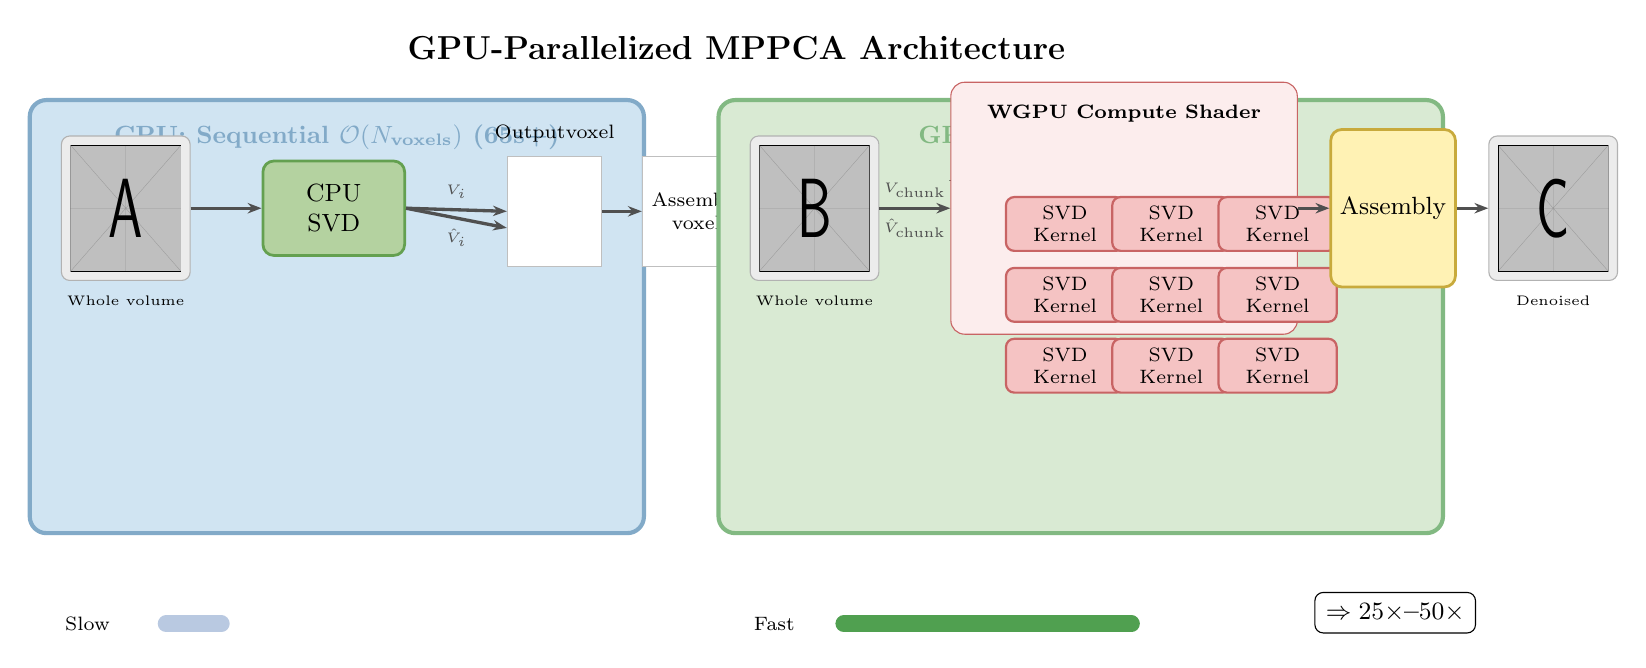
\begin{tikzpicture}[node distance=0.5cm]

%% ═══════════════════════════════════════════════════════════════════
%%  TOP TITLE
%% ═══════════════════════════════════════════════════════════════════
\node[font=\large\bfseries, anchor=north] (title) at (9,0.3)
  {GPU-Parallelized MPPCA Architecture};

%% ═══════════════════════════════════════════════════════════════════
%%  LEFT PANEL  –  CPU (Sequential)
%% ═══════════════════════════════════════════════════════════════════

% Panel background
\begin{scope}
  \node[panelBox, draw=cpuBorder, fill=cpuBlue,
        minimum width=7.8cm, minimum height=5.5cm,
        anchor=north west] (cpuPanel) at (0,-0.6) {};

  \node[font=\small\bfseries, text=cpuBorder, anchor=north]
    at (cpuPanel.north) [yshift=-6pt]
    {CPU: Sequential $\mathcal{O}(N_\text{voxels})$ (65s+)};

  % "Exit" label top-left
  \node[font=\scriptsize, anchor=north west] at (cpuPanel.north west) [xshift=14pt,yshift=-22pt]
    {\textit{Exit}};

  % Brain scan (input)
  \node[brainImg, anchor=west] (brainCPU) at ([xshift=12pt]cpuPanel.west |- 0,-2.0)
    {\includegraphics[width=1.4cm,height=1.6cm]{example-image-a}};
  \node[font=\tiny, below=2pt of brainCPU] {Whole volume};

  % CPU SVD box
  \node[cpuBox, right=0.9cm of brainCPU] (cpuSVD)
    {CPU\\SVD};

  % Output voxel label + box
  \node[font=\scriptsize, above right=0.1cm and 1.0cm of cpuSVD, anchor=south west]
    (outVoxLabel) {Output\\voxel};
  \node[voxelBox, below=0.05cm of outVoxLabel] (outVox) {};

  % Assemble voxel box
  \node[voxelBox, right=0.5cm of outVox] (assVox)
    {\scriptsize Assemble\\voxel};

  % Arrows CPU path
  \draw[mainArrow] (brainCPU.east) -- (cpuSVD.west);
  \draw[mainArrow] (cpuSVD.east) -- (outVox.west)
    node[midway, above, font=\tiny] {$V_i$};
  \draw[mainArrow] (cpuSVD.east) -- ([yshift=-6pt]outVox.west)
    node[midway, below, font=\tiny] {$\hat{V}_i$};
  \draw[mainArrow] (outVox.east) -- (assVox.west);

  % Speed bar
  \node[font=\scriptsize, anchor=west] (slowLabel) at ([xshift=10pt,yshift=-32pt]cpuPanel.south west)
    {Slow};
  \draw[speedBar, color=slowBlue!40]
    ([xshift=50pt,yshift=-32pt]cpuPanel.south west) --
    ([xshift=70pt,yshift=-32pt]cpuPanel.south west);
\end{scope}

%% ═══════════════════════════════════════════════════════════════════
%%  RIGHT PANEL  –  GPU (Parallel)
%% ═══════════════════════════════════════════════════════════════════
\begin{scope}
  \node[panelBox, draw=gpuBorder, fill=gpuGreen,
        minimum width=9.2cm, minimum height=5.5cm,
        anchor=north east] (gpuPanel) at (18,-0.6) {};

  \node[font=\small\bfseries, text=gpuBorder, anchor=north]
    at (gpuPanel.north) [yshift=-6pt]
    {GPU: Parallel $\mathcal{O}(1)$ ($<$2s)};

  % "Exit" / "Extract" labels
  \node[font=\scriptsize, anchor=north west] at (gpuPanel.north west) [xshift=14pt,yshift=-22pt]
    {\textit{Exit}};
  \node[font=\scriptsize, anchor=north west] at (gpuPanel.north west) [xshift=80pt,yshift=-22pt]
    {\textit{Extract}};

  % Brain scan (input)
  \node[brainImg, anchor=west] (brainGPU) at ([xshift=12pt]gpuPanel.west |- 0,-2.0)
    {\includegraphics[width=1.4cm,height=1.6cm]{example-image-b}};
  \node[font=\tiny, below=2pt of brainGPU] {Whole volume};

  % WGPU shader box (contains SVD kernels)
  \node[draw=shaderBorder, fill=shaderPink!30, rounded corners=5pt,
        minimum width=4.4cm, minimum height=3.2cm,
        right=0.9cm of brainGPU, anchor=west] (wgpuBox) {};
  \node[font=\scriptsize\bfseries, anchor=north] at (wgpuBox.north) [yshift=-5pt]
    {WGPU Compute Shader};

  % 3x3 grid of SVD kernels
  \foreach \row in {1,2,3} {
    \foreach \col in {1,2,3} {
      \node[svdKernel] at
        ([xshift={\col*1.35cm-2.1cm}, yshift={-\row*0.9cm+0.7cm}]wgpuBox.center)
        (svd\row\col) {\scriptsize SVD\\Kernel};
    }
  }

  % Assembly box
  \node[assemblyBox, right=0.4cm of wgpuBox] (assembly) {Assembly};

  % Denoised brain
  \node[brainImg, right=0.4cm of assembly] (brainOut)
    {\includegraphics[width=1.4cm,height=1.6cm]{example-image-c}};
  \node[font=\tiny, below=2pt of brainOut, align=center] {Denoised};

  % Arrows GPU path
  \draw[mainArrow] (brainGPU.east) -- (wgpuBox.west)
    node[midway, above, font=\tiny] {$V_\text{chunk}$}
    node[midway, below, font=\tiny] {$\hat{V}_\text{chunk}$};
  \draw[mainArrow] (wgpuBox.east) -- (assembly.west);
  \draw[mainArrow] (assembly.east) -- (brainOut.west);

  % Speed bar + speedup badge
  \node[font=\scriptsize, anchor=west] (fastLabel) at ([xshift=10pt,yshift=-32pt]gpuPanel.south west)
    {Fast};
  \draw[speedBar, color=fastGreen]
    ([xshift=46pt,yshift=-32pt]gpuPanel.south west) --
    ([xshift=150pt,yshift=-32pt]gpuPanel.south west);

  % Speedup badge
  \node[draw=black, fill=white, rounded corners=3pt,
        font=\small\bfseries, inner sep=4pt]
    at ([xshift=-18pt,yshift=-28pt]gpuPanel.south east)
    {$\Rightarrow 25\times$--$50\times$};
\end{scope}

\end{tikzpicture}
\end{document}
